\subsection{Esecuzione dell'esperienza}

La prima operazione fatta è stata quella di verificare il corretto allineamento dell'interferometro. Abbiamo infatti notato che se i due specchi non sono perpendicolari tra loro, sullo schermo si vedono figure di interferenza complicate e difficili da trattare invece che una semplice figura di interferenza lineare in cui si alternano massimi e minimi. Per allineare lo strumento è sufficiente ruotare delicatamente i due specchi finché non compare sullo schermo una figura d'interferenza semplice.

%Facciamo notare che nonostante l'attenzione prestata, lo specchio e lo schermo non sono risultati essere perfettamente paralleli tra di loro. Questo comporta che i due raggi luminosi incidenti sullo schermo non sono allineati tra di loro. Infatti sullo schermo si visualizzano in alternanza delle frange di interferenza costruttiva e distruttiva, ovvero picchi luminosi e non che si alternano con regolarità.
% WTF????

La misura dell'indice di rifrazione di un dato materiale con l'interferometro di Michelson si esegue adottando la seguente strategia.
Si parte da una configurazione base, per esempio l'interferometro con un ramo su cui e già stata montata la camera da vuoto
(si veda la Figura \ref{fig:mik}). A questo punto sullo schermo è proiettata una figura di interferenza. Dopodiché si
varia gradualmente un qualche parametro del materiale sotto esame, per esempio la pressione (nel caso dell'aria), la lunghezza o l'inclinazione (per il vetro) oppure la concentrazione (per una soluzione). % beh, la soluzione è dell'esperimento successivo...
Questo serve per variare il cammino ottico del raggio che attraversa il materiale.
In questo modo la figura di interferenza varia e le frange si muovono. Dal conteggio delle frange si riesce ad ottenere, mediante
apposite formule, l'indice di rifrazione voluto.

%La seguente relazione lega il numero $N$ di frange passate sullo schermo, alla differenza di cammino ottico $d$.

%\begin{equation}
%    N \,=\, \frac{d}{\lambda} = \frac{\Delta n \cdot 2 \ell}{\lambda}
%\end{equation}
%
%Nella formula $\lambda$ indica la lunghezza d'onda della luce, $\Delta n$ la differenza di indice di rifrazione tra la configurazione base e quella attuale, mentre $2\ell$ e la lunghezza della camera (il 2 serve perché la luce attraversa la camera due volte).

%Una volta giunti al valore di pressione, lunghezza concentrazione voluto,


\begin{SCfigure}[0.70][t]
    \centering
    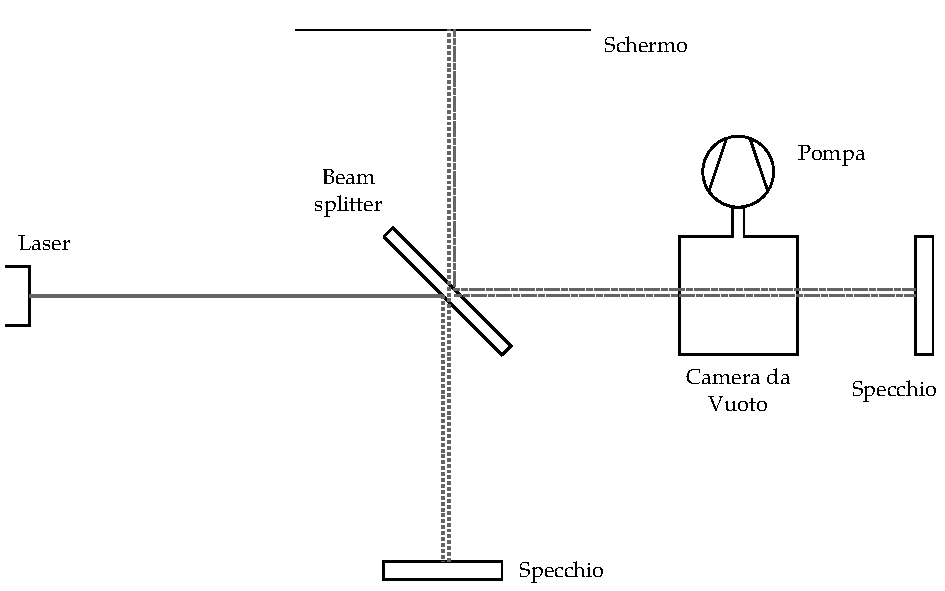
\includegraphics[width=120mm]{drawing.pdf}
    \caption{Schema semplificato del sistema utilizzato per misurare l'indice di rifrazione dell'aria.}
    \label{fig:mik}
\end{SCfigure}

\subsubsection{Indice di rifrazione dell'aria}

La procedura eseguita per ricavare l'indice di rifrazione dell'aria è la seguente:

\begin{itemize}
	\item{Abbiamo installato sul sistema, tra il beam splitter e lo specchio mobile, una piccola camera da vuoto con due pareti in vetro atte a far passare la luce % diggiuro!
	 e la camera è stata collegata, mediante la valvola a spillo, alla pompa a membrana;}
    \item{Partendo con la camera da vuoto a pressione atmosferica abbiamo man mano creato il vuoto all'interno della camera regolando l'apertura della valvola a spillo. Aprendo la valvola a spillo (ovviamente con la pompa accesa), l'aria esce dalla camera da vuoto ed esce in atmosfera;}
    \item{Ad intervalli regolari di pressione, ovvero ogni \SI{10}{\kilo\pascal}, abbiamo annotato il numero di frange di interferenza passate sullo schermo;}
\end{itemize}

\subsubsection{Indice di rifrazione del vetro}

Per misurare l'indice di rifrazione del vetro abbiamo adottato una strategia simile. Dobbiamo partire da una data figura di interferenza e variare il cammino ottico di uno dei due raggi, contando il numero di massimi di intensità, ovvero il numero delle frange.

Ponendo un vetro tra il beam splitter e lo specchio fisso si tara lo strumento. Per variare poi il cammino ottico abbiamo
inclinato il vetro; in questo modo la sezione che viene attraversata dal raggio è maggiore e varia il cammino ottico.
Inoltre il raggio luminoso è costretto ad attraversare il vetro sia in ``andata'' che al ``ritorno''.

Abbiamo iniziato allineando il vetro in modo che fosse perpendicolare al raggio. Si è posto il raggio su di un goniometro posto
tragitto del raggio. Ruotando il goniometro è stato cercato l'angolo per cui la figura di diffrazione si fermasse e tornasse indietro.
Questo è l'angolo per cui il vetro è perpendicolare al raggio ed il cammino ottico è minore.
%Pertanto, dopo aver posizionato il vetro,
%si agisce sullo specchio mobile allontanandolo o avvicinandolo al beam spltte per allinearlo con lo specchio fisso. Si fa questo al fine di ottenere una semplice figura di interferenza, che come nel caso precedente è una frangia luminosa.

A questo punto si segna l'angolo di allineamento, che nel nostro caso ha il seguente valore:

\begin{equation}
	\theta_0 \,=\, 2.2 \pm 0.1
\end{equation}
%
Ruotando lo specchio ad ampiezze sempre maggiori si varia il cammino ottico del raggio luminoso rifratto.
In tal modo scorre sullo schermo un certo numero di frange, il quale varia non linarmente con l'aumentare dei gradi.

\subsection{Analisi Dati}

Per ricavare gli indici di rifrazione abbiamo sfruttato la seguente legge:

\begin{equation}
	N \,=\, \frac{d}{\lambda}
\end{equation}
%
dove con $N$ si indica il numero di frange (massimi di intensità) contati, $d$ la differenza di cammino
ottico tra la configurazione base e quella raggiunta e $\lambda$ la lunghezza d'onda del laser.

\subsubsection{Indice di rifrazione dell'aria} %: quadro teorico}

% non è proprio vero...
%Ricordiamo che a condizione di pressione costante il cammino ottico percorso dai due raggi luminosi risulta essere lo stesso.
Lo scopo sarà quello di confrontare il numero di frange contate con la differenza di pressione rilevata.
Infatti variando la pressione nella camera da vuoto si varia l'indice di rifrazione dell'aria.
Questo provoca una variazione nel cammino ottico del raggio  e quindi fenomeni di interferenza.
Tali fenomeni saranno sempre più accentuati man mano che l'indice di rifrazione dell'aria varia in funzione della pressione interna alla camera.
Sapendo che il cammino ottico ($D$) è pari a due volte la lunghezza della camera da vuoto moltiplicata per l'indice di rifrazione del gas ivi contenuto, possiamo ottenere la seguente relazione:

\begin{equation}
	\Delta{n} \,=\, \frac{N \, \lambda}{D} \qquad \text{con} \qquad \Delta{n} \,=\, (n\ped{p} \,-\, n\ped{vuoto})
	\label{eq:delta_n}
\end{equation}
%
dove $n\ped{p}$ è l'indice di rifrazione dell'aria alla pressione raggiunta, $n\ped{vuoto}$ è l'indice di rifrazione del vuoto il cui valore è 1 preso senza incertezze, $D$ la differenza di cammino ottico tra i due raggi e $\lambda$ e la lunghezza d'onda del laser.

Quindi per ottenere il valore dell'idice di rifrazione dell'aria alla pressione voluta non dobbiamo fare altro che isolare dall'equazione (\ref{eq:delta_n}) il tremine $n\ped{p}$. Pertanto otteniamo che:

\begin{equation}
	n\ped{p} \,=\, 1 \,+\, \frac{N \, \lambda}{D}
	\label{eq:indice_rif_aria}
\end{equation}
%
e quindi grazie all'interpolazione dei dati del numero di frange contate ($N$) in funzione della pressione raggiunta ($P$) possiamo ricavere il numero di massimi ($N\ped{atm}$) relativi alla pressione atmosferica ($P\ped{atm}$).
Infine sfruttando la precedente relazione (\ref{eq:indice_rif_aria}) siamo in grado di ottenere il valore dell'indice di rifrazione dell'aria a pressione atmosferica:

\begin{equation}
	n\ped{patm} \,=\, 1 \,+\, \frac{N\ped{atm} \, \lambda}{D}
	\label{eq:indice_rif_aria_atm}
\end{equation}
%

%Quindi ora avendo il quadro teorico che sta alla base dell'esperimento possiamo procedere con l'analizzare i dati che abbiamo ottenuto.
Il valore da noi ricavato per l'indice di rifrazione è:

\begin{equation}
	n\ped{atm} \, = \, 1.00020 \pm 0.00001
\end{equation}

L'indice di rifrazione dell'aria a pressione atmosferica e a temperatura di 20 $\si{\degreeCelsius}$ reperibile in letteratura è\footnote{Il valore è stato preso da it.wikipedia.org/wiki/Indice\_di\_rifrazione}:
\begin{equation}
n\ped{atm} \, = \, 1.000 292 6
\end{equation}

Il nostro valore è lontano da quello misurato da gente seria e non è neanche lontanamente compatibile. Evidentemente la nostra incertezza
è ridicola, poiché si basa quasi solamente sull'incertezza del conteggio e su quella dello spessore della camera che sono entrambe inverosimilmente piccole. In particolare l'incertezza di conteggio deriva dalla fluttuazione statistica dei valori delle serie, che essendo poco numerosi portano ad un'incertezza troppo piccola.

%\subsubsection{Valore indice di rifrazione dell'aria}

\begin{figure}[t]
    \centering
%		[b]{0.3\textwidth}
        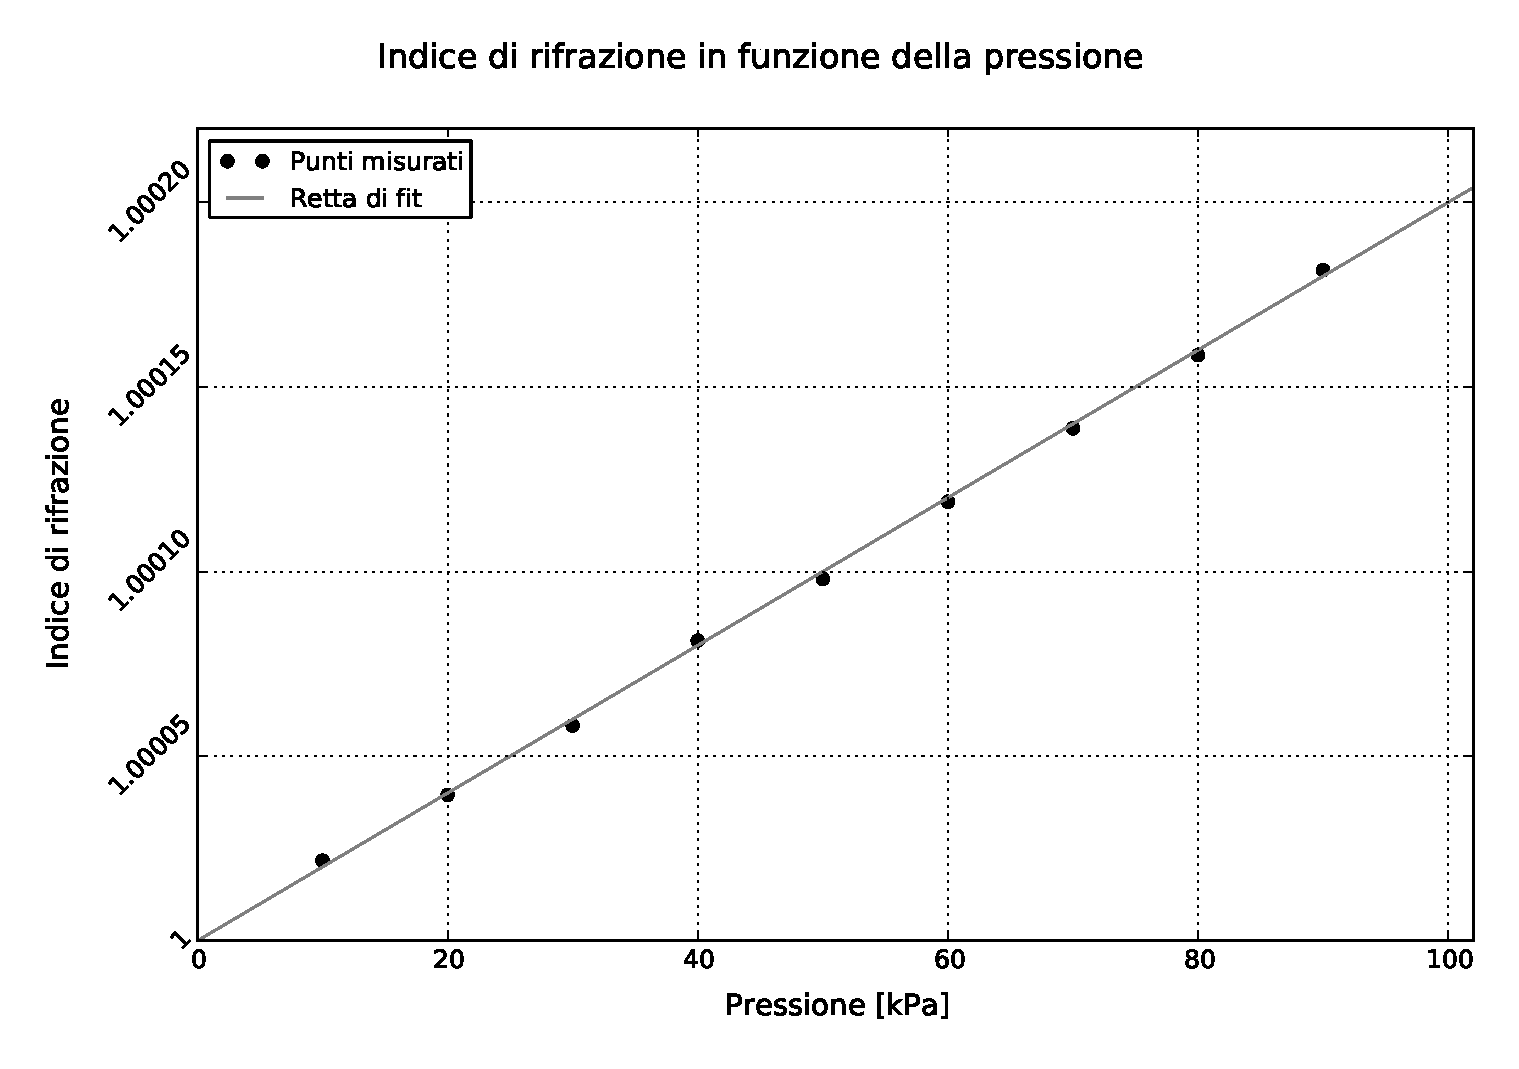
\includegraphics[width=\textwidth]{graph.pdf}
        \caption{Indice di rifrazione dell'aria in funzione della pressione. La relazione è lineare e si vede che, a pressione
			atmosferica, l'indice di rifrazione è precisamente 1.0002.}
        \label{fig:enne_press}
\end{figure}

\subsubsection{Indice di rifrazione del vetro}


Lo schema in Figura \ref{fig:mik} rappresenta ancora il tavolo di lavoro ad eccezione che al posto della camera da vuoto abbiamo posizionato un vetro dello spessore di circa 6 \si{\milli\metre} su uno specifico supporto girevole.

Per ricavare l'indice di rifrazione del vetro abbiamo usato un procedimento del tutto simile a quello descritto nel paragrafo precedente.
Se però per l'aria variavamo la sua pressione tramite una pompa ed una valvola a spillo, ora ruotiamo il vetro in modo tale che il raggio di luce compia un tragitto maggiore nel vetro. % fa un po' schifo sta frase...

Grazie a \emph{banali} calcoli di ottica geometrica si riesce \emph{immediatamente} a dedurre l'equazione che lega l'indice di rifrazione del vetro all'angolo (e quindi alla differenza di cammino ottico e alle frange contate). Tale \emph{elementare} relazione è:
\begin{equation}
	n\ped{vetro} \, = \, \frac{(2t - N \lambda) (1 - cos(\theta))}{2t(1-cos(\theta))-N\lambda}
\end{equation}
dove $t$ è la lunghezza del vetro, $\lambda$ è la lunghezza d'onda, $\theta$ è la rotazione del vetro rispetto al fascio di luce
($\theta = 0$ equivale al raggio perpendicolare al vetro)
e $N$ è il numero di frange contate tra $\theta_0$ e la successiva posizione.
I valori costanti nel nostro caso sono $t \,=\, 5.75 \pm 0.05 \, mm$ e $\lambda \, = \, 543.5 \, \si{\nano\metre}$.

I nostri dati hanno portato, tramite la media pesata dei dati ricavati ad ogni $\theta$, ad ottenere il seguente valore:
\begin{equation}
	n\ped{vetro} \, = \, 1.59 \pm 0.01
\end{equation}

\begin{figure}[t]
    \centering
        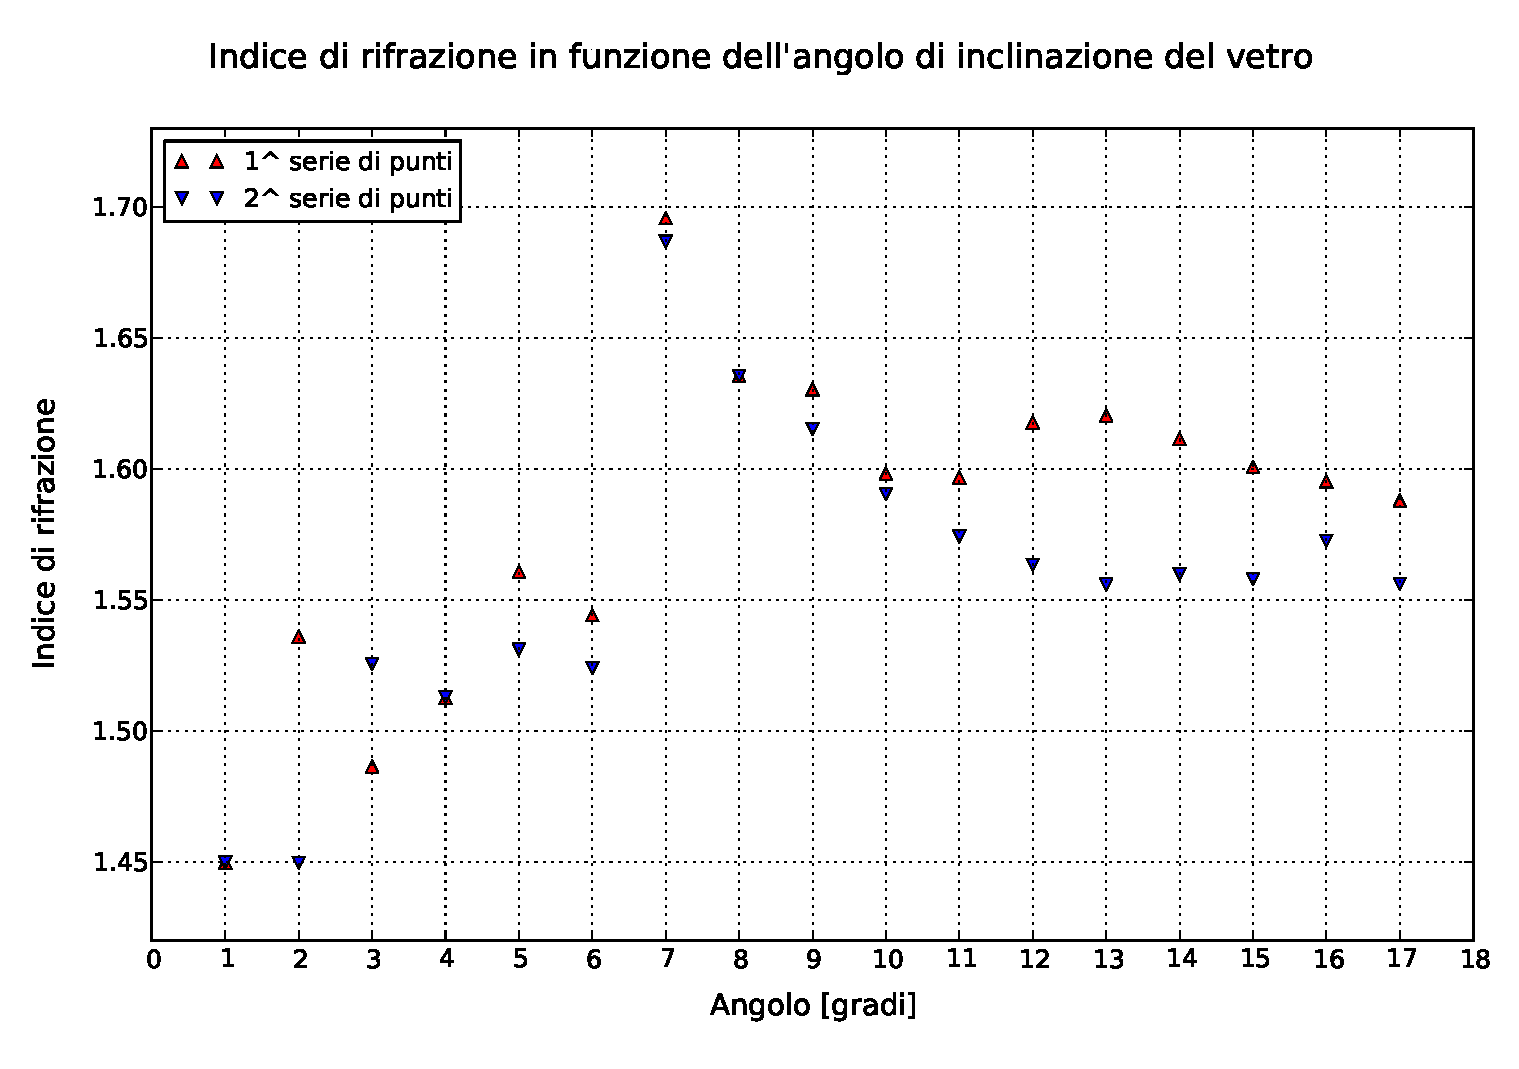
\includegraphics[width=\textwidth]{lol.pdf}
        \caption{Indice di rifrazione del vetro in funzione dell'angolo.}
        \label{fig:enne_theta}
\end{figure}
